% This must be in the first 5 lines to tell arXiv to use pdfLaTeX, which is strongly recommended.

\pdfoutput=1
% In particular, the hyperref package requires pdfLaTeX in order to break URLs across lines.
\pdfminorversion=7
\pdfobjcompresslevel=3
\pdfcompresslevel=9

\documentclass[11pt]{article}
\usepackage{graphicx}
% Change "review" to "final" to generate the final (sometimes called camera-ready) version.
\usepackage{acl}

% pour gérer les figures et tableaux avec H
\usepackage{float}
% tableaux plus propres
\usepackage{booktabs}

% Standard package includes
\usepackage{times}
\usepackage{latexsym}

% For proper rendering and hyphenation of words containing Latin characters (including in bib files)
\usepackage[T1]{fontenc}

% This assumes your files are encoded as UTF8
\usepackage[utf8]{inputenc}

\usepackage{amsmath}

% This is not strictly necessary, and may be commented out,
% but it will improve the layout of the manuscript,
% and will typically save some space.
\usepackage{microtype}

% This is also not strictly necessary, and may be commented out.
% However, it will improve the aesthetics of text in
% the typewriter font.
\usepackage{inconsolata}

%Including images in your LaTeX document requires adding
%additional package(s)
\usepackage{graphicx}

% pour mettre une en-tête et des pieds de pages
\usepackage{fancyhdr}
\pagestyle{fancy}

% Réinitialise les en-têtes et pieds de page
\fancyhf{} 
% En-tête au centre [C] mais sinon [L][R] pour gauche droite
\fancyhead[L]{\textit{DEFT’09 « DÉfi Fouille de Textes », Paris, 6 janvier 2025}}

% Enlever la barre horizontale
\renewcommand{\headrulewidth}{0pt} 

% pour la pagination automatique
\fancyfoot[R]{\thepage}
% pour forcer la pagination sur la première page
\thispagestyle{fancy}

\title{DEFT'09 : classifier automatiquement les groupes politiques}

\author{
  \text{MANSERI Kéhina\textsuperscript{(1)(2)}}
  \text{SIRVEN-VIENOT Alix\textsuperscript{(1)(2)}}
  \text{VAN-DEN-ZANDE Débora\textsuperscript{(1)(3)}}
\\
\\
  \textsuperscript{(1)}Université Paris Nanterre
  \textsuperscript{(2)}Parcours Recherche et Développement
  \textsuperscript{(3)}Parcours Pro
\\
\\
    \small {
    manserikehina@gmail.com, alix.vienot@gmail.com, vdzdebora@gmail.com
    }
\\
}

\begin{document}
\maketitle

\begin{abstract}

Cet article présente un travail consistant en la classification automatique d'interventions parlementaires en fonction du parti politique. Le corpus analysé est multilingue et présente des défis liés au déséquilibre des classes et à la diversité des thématiques abordées. Cet article illustre la manière dont certains classifieurs et stratégies d'équilibrage des données peuvent être mieux adaptés à une tâche et à un corpus présentant des spécificités similaires aux nôtres.

% This article presents work involving the automatic classification of parliamentary interventions based on political party affiliation. The analyzed corpus is multilingual, including interventions in French, English, and Italian. It also presents challenges related to class imbalance and to the diversity of topics addressed. This article illustrates how certain classifiers and data balancing strategies can be better suited to a task and a corpus with specific characteristics similar to ours.

\end{abstract}

\section{Introduction}

Ce travail s'inscrit dans la continuité des expériences menées dans le cadre de la \textbf{tâche 3 du Défi Fouille de Textes 2009} pour laquelle uniquement une équipe de recherche avait publié ses résultats \cite{forest2009variation}. Nous nous baserons sur ces derniers pour justifier certains choix et juger les performances de modèles sur le corpus français.

Nous commencerons par présenter notre corpus ainsi que les pré-traitements appliqués aux données. Nous introduirons ensuite les algorithmes et statégies utilisés pour effectuer plusieurs prédictions. Enfin, nous analyserons les résultats obtenus et établirons les éléments semblant contribuer aux meilleures performances.

Vous pouvez retrouver l'entierté du code rédigé sur notre GitHub\footnote{\url{https://github.com/KehinaleK/deft09/tree/main}}.


% PRÉSENTATION DES DONNÉES !!!


\section{Présentation des données}
Les corpus fournis sont comparables et disponibles en : français, anglais, et italien. Les ensembles d'entraînement et de test composant chaque corpus contiennent les mêmes interventions mais dans un ordre différent. 

\subsection{Extraction des données}
Les données ont été téléchargées sur le site du DEFT\footnote{\url{https://deft.lisn.upsaclay.fr/}} et parsées afin d'extraire les données de chaque ensemble. 

\subsection{Suppression des doublons}
Après concertation avec les autres participants, nous avons été informées que les ensembles d'entraînement et de test présentaient des doublons. Nous avons pu trouver 7 813 interventions concernées.

Nous avons donc décidé de retirer ces doublons de manière alternée entre les deux ensembles puis uniquement de l'ensemble de test afin de rester le plus proche possible de la division originale du corpus en 60\% d'échantillons d'entraînement et 40\% de test. \textbf{Nous avons ainsi pu atteindre une répartition exacte de 60\% (13 068) et 40\% (8 712).}

\subsection{Distribution des classes}
Après suppression des doublons et équilibrage de la division, nous obtenons la répartition de classes suivante : (cf. Tableau~\ref{tab:pourcentage_test}).

\begin{table}[ht]
\centering
    \begin{tabular}{lccc}
        \toprule
        \textbf{Classe}   & \textbf{Train} & \textbf{Test} & \textbf{Pourcentage} \\ \midrule
        \textbf{PSE}      & 3 650           & 2 489          & 40.54\% \\    
        \textbf{ELDR}     & 1 351           & 908           & 40.19\% \\          
        \textbf{Verts-ALE}& 1 609           & 1 072          & 39.99\% \\          
        \textbf{PPE-DE}   & 4 635           & 3 047          & 39.66\% \\          
        \textbf{GUE-NGL}  & 1 823           & 1 196          & 39.62\%  \\ 
        \bottomrule            
    \end{tabular}
    \caption{Distribution des pourcentages entre Train et Test.}
    \label{tab:pourcentage_test} % Tableau~\ref{tab:pourcentage_test}
\end{table}

% \textbf{Résumé des totaux} \\
% Total Train : \> 13068 \\
% Total Test  : \> 8712 \\
% Pourcentage Global Test : \> 40.00\%
% \\

À première vue, les classes semblent déséquilibrées. Cette disparité des classes dans les deux ensembles est présentée sur la Figure~\ref{fig:graph_avant}.

\begin{figure}[H]
  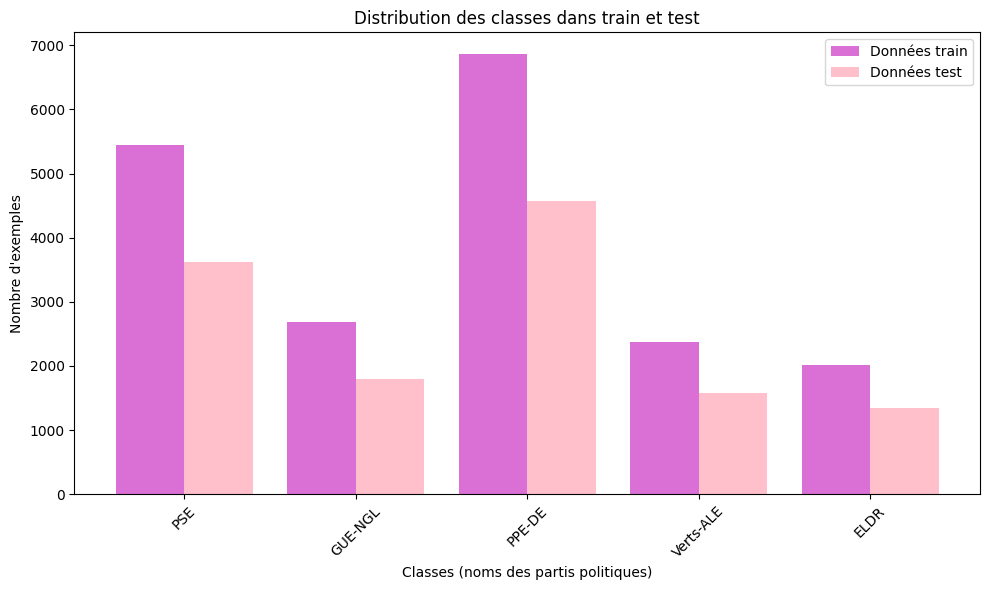
\includegraphics[width=\columnwidth]{latex/graphique_avant.png}
  \caption{Répartition des classes \textbf{avant} suppression des doublons.}
  \label{fig:graph_avant} % pareil pour citer Figure~\ref{fig:graph_avant}
\end{figure}



\begin{figure}[H]
  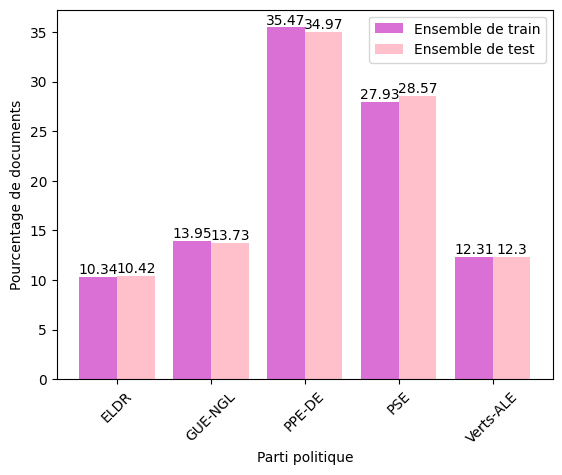
\includegraphics[width=\columnwidth]{latex/graphique_apres.png}
  \caption{Répartition des classes \textbf{après} suppression des doublons.}
  \label{fig:graph_apres} % Figure~\ref{fig:graph_apres}
\end{figure}


\section{Pré-traitement des données}
\subsection{Normalisation des données}
Nous avons appliqué plusieurs étapes de normalisation aux données : la ponctuation et les \textit{stopwords} ont été supprimés, tous les textes ont été convertis en minuscules pour uniformiser leur format. Enfin, une lemmatisation a été effectuée pour ramener les mots à leur forme canonique, optimisant ainsi la cohérence des données textuelles.

\subsection{Vectorisation des données}
Les essais menés par les participants précédents à la tâche 3 montrent que les hyperparamètres utilisés lors de la vectorisation des données jouent un rôle dans l'amélioration des résultats.

En se basant sur ces essais et les conclusions présentées dans le TP1\cite{TP1}, 11 vectorisations TfIdf ont été appliquées sur nos données avec des valeurs d'hyperparamètres différentes. La taille du vocabulaire retenu, la taille des ngrammes analysés, et le seuil accepté du nombre de documents. 

Nous avons ensuite procédé à des essais sur trois classifieurs basés sur des concepts différents et avec leurs hyperparamètres par défaut : KNN (car utilisé dans l'article) SVC Lineaire (modèle linéaire) et Complement NB (modèle probabilistique).

Si nous ne pouvons pas affirmer avec certitude qu'une vectorisation plus performante en utilisant trois algorithmes le sera aussi pour les autres, nous avons décidé d'utiliser celle nous donnant les meilleures valeurs de macro f-mesure et d'accuracy pour le reste de nos tests.

\begin{table}[ht]
\centering
\resizebox{\columnwidth}{!}{%
    \begin{tabular}{lccccc}
        \toprule
        \textbf{Algorithme}   & \textbf{Accuracy} & \textbf{f-mesure} & \textbf{Précision} & \textbf{Rappel} \\ \midrule
        \textbf{KNN} & 0.349 & 0.272 & 0.288 & 0.275 \\    
        \textbf{CompNB} & 0.38 & 0.32 & 0.332 & 0.366 \\
        \textbf{LinearSVC} & 0.418 & 0.331 & 0.393 & 0.329 \\          
        \bottomrule            
    \end{tabular}%
}
\caption{Meilleurs résultats obtenus pour chaque algorithme.}
\label{tab:pourcentage_test}
\end{table}


Les vectorisations permettant d'obtenir les meilleurs résultats pour le LinearSVC et le KNN sont les mêmes : \textbf{max\_df de 0.5, ngram\_range de (1, 2) et un max\_features illimité.} Les résultats obtenus pour cette vectorisation restant elevés pour le ComplementNB, nous avons décidé d'utiliser cette dernière pour les essais suivants. Le même test a également été réalisé en utilisant les données non normalisées sans qu'une grande différence n'ait pu être observée. Nous avons donc poursuivi nos tests avec les données normalisées car moins volumineuses.

\section{Comparaison des algorithmes}
 Nous avons utilisé un ensemble d'algorithmes basés sur des concepts différents et avec des combinaisons variées d'hyperparamètres (cf. Tableau~\ref{tab:classifieurs_types}).


\begin{table}[h]
    \centering
    \begin{tabular}{|l|l|}
        \hline
        \textbf{Nom du Classifieur}        & \textbf{Type} \\ \hline
        LinearSVC                         & Linéaire      \\ \hline
        RandomForestClassifier            & Ensemble      \\ \hline
        KNeighborsClassifier              & Non-linéaire  \\ \hline
        PassiveAggressiveClassifier       & Linéaire      \\ \hline
        MultinomialNB                     & Probabiliste  \\ \hline
        ComplementNB                      & Probabiliste  \\ \hline
        SVC                               & Non-linéaire  \\ \hline
        RidgeClassifier                   & Linéaire      \\ \hline
        LGBMClassifier                    & Ensemble      \\ \hline
        LogisticRegression                & Linéaire      \\ \hline
        SGDClassifier                     & Linéaire      \\ \hline
    \end{tabular}
    \caption{Liste des classifieurs et leur type.}
    \label{tab:classifieurs_types} % ça c'est pour le citer après ! Tableau~\ref{tab:classifieurs_types}
\end{table}

\subsection{Choix des algorithmes}
Au vu des conclusions effectuées lors de la campagne initiale du défi, nous savions en effet que les résultats obtenus en utilisant KNN et des méthodes bayesiennes ne dépassaient pas les 33.9 pour la macro f-mesure. 
Des modèles linéaires (LinearSVC, RidgeClassifier), généralement plus limités dans un contexte similaire au nôtre, ont été comparés à des modèles probabilistes (MultinomialNB, ComplementNB) et ensemblistes (Random Forest, LGBMClassifier), connus pour leur aptitude à mieux gérer les données déséquilibrées.

\subsection{Choix des hyperparamètres}
Pour tenter de s'adapter au mieux à nos données, nous avons notamment utilisé plusieurs fonctions de perte pour le SGDClassifier et le PassiveAggressiveClassifier \cite{PassiveAgressiveC} ainsi que des kernels différents pour les SVC.

\section{Stratégies d'amélioriation}

Afin de pousser la comparaison de différents modèles, nous avons décidé d'avoir recours à quelques essais supplémentaires permettant de contrer le déséquilibre de nos classes. 

\subsection{Sous et sur-échantillonnage}
Nous avons premièrement utilisé le sous-échantillonnage et le sur-échantillonnage, des techniques consistant en la duplication ou la division du nombre d'échantillons de chaque classe. Avoir une distribution de classe équilibrée est essentielle car permettant en général au modèle de performer de manière similaire sur toutes les classes.

Dans notre cas, les classes sous-représentées peuvent mener à des scores de rappel et de précision très bas, contrairement aux classes majoritaires. 

Nous avons donc ré-entrainé l'ensemble de nos modèles sur nos données après sous-échantillonnage et sur-échantillonnage. 
\begin{figure}[H]
  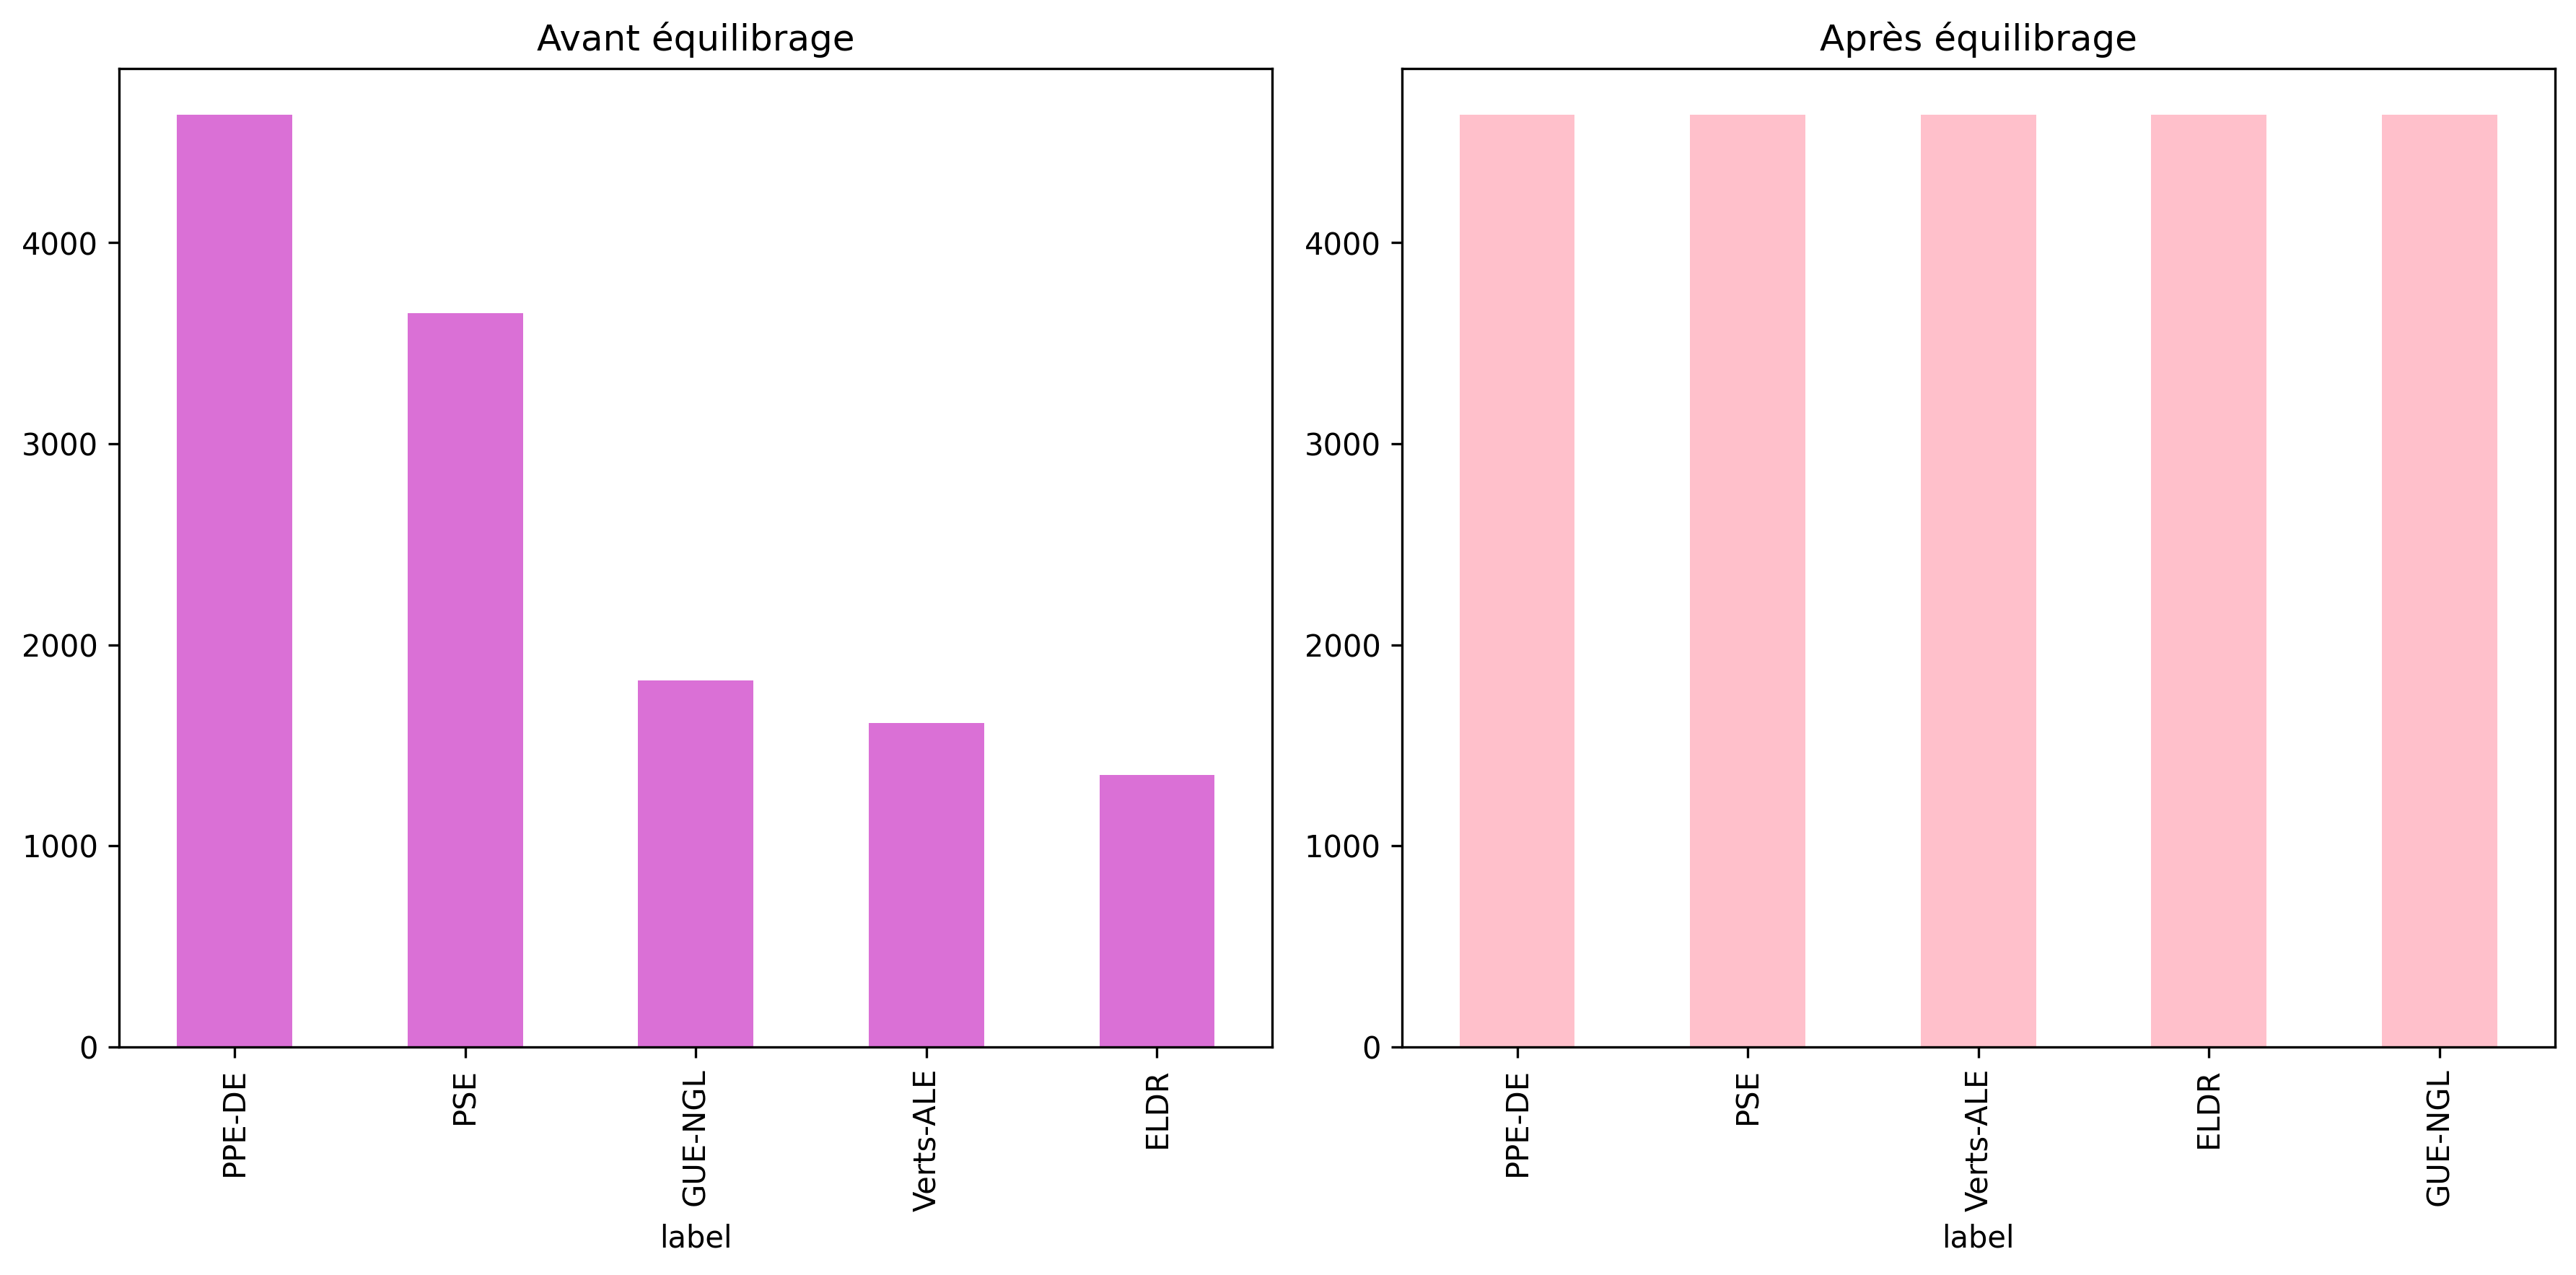
\includegraphics[width=\columnwidth]{latex/equilibrage.png}
  \caption{Répartition des classes \textbf{avant} et \textbf{après} sur échantillonnage.}
  \label{fig:equilibrage} % pareil pour citer Figure~\ref{fig:equilibrage}
\end{figure}

\subsection{Utilisation des corpus comparables}
Enfin, nous avons décidé d'utiliser les corpus italien et anglais (après suppression des doublons) pour entraîner de nouveau chaque modèle.

En effet, nous pensions intéressant d'utiliser ces derniers pour augmenter le volume de notre corpus d'entraînement pour ensuite prédire uniquement les labels des échantillons français. 

\section{Évaluation des modèles}

Une fois les modèles entrainés, nous avons cherché à évaluer leurs prédictions de manière pertinente.

\subsection{Métriques d'évaluation}

\textbf{Nous avons décidé de prendre en compte la macro f-mesure plutôt que l'accuracy.} 

Si la seconde rend compte du nombre de bonnes prédictions sur le total de prédictions, la première permet elle d'apporter la même importance à chaque classe en faisant la somme des valeurs de précision et de rappel de ces dernières. 

Elle permet notamment de juger un modèle sur sa capacité à classifier les échantillons de toutes les classes et de ne pas réduire l'impact des scores moins bons des classes minoritaires lorsque ceux des classes majoritaires sont plus élevés.

\subsection{Résultats pour les données initiales}

\begin{table}[ht]
\centering
\resizebox{\columnwidth}{!}{%
    \begin{tabular}{lccccc}
        \toprule
        \textbf{Algorithme}   & \textbf{Accuracy} & \textbf{f-mesure} & \textbf{Précision} & \textbf{Rappel} \\ \midrule
        \textbf{Passive Aggressive} & 0.412 & 0.344 & 0.375 & 0.339 \\    
        \textbf{LinearSVC} & 0.418 & 0.331 & 0.393 & 0.329 \\
        \textbf{SGDC} & 0.336 & 0.32 & 0.33 & 0.362 \\ 
        \bottomrule            
    \end{tabular}%
}
\caption{Meilleurs résultats obtenus sur les données initiales.}
\label{tab:pourcentage_test}
\end{table}

En se basant donc sur les valeurs de macro f-mesure, les modèles les plus performants sont: \textbf{Passive Aggressive Classifier} (avec valeur de paramètre de régularisation de 0.5 et la fonction de perte squared hinge), le \textbf{LinearSVC} (avec une formulation duale) et le \textbf{SGDClassifier} (avec ses hyperparamètres par défaut).

Le PassiveAggressiveClassifier reste en réalité plus efficace que le LinearSVC et le SGDClassifier peu importe ses valeurs d'hyperparamètres mais nous avons ici décidé de présenter les trois meilleurs algorithmes. 

Nous pouvons premièrement voir que les valeurs de macro f-mesure restent très proches dans les trois cas. Si le score d'accuracy du SGDC s'avère clairement moins bon que ceux des deux autres modèles, il reste très proche de sa propre macro f-mesure. Il semblerait donc ici que le SGDC permette d'obtenir des prédictions plus similaires entre chaque classe mais moins bonnes en moyenne pour chacune d'entre elles là ou le LinearSVC et le PassiveAggressiveClassifier prédisent mieux certaines classes mais bien moins d'autres.

\subsection{Résultats pour le sur-échantillonnage}

Nous avons ensuite entrainé ces trois classifieurs sur les données obtenues après un sur-échantillonnage pour voir si des différences de scores pouvaient être observées.

\begin{table}[ht]
\centering
\resizebox{\columnwidth}{!}{%
    \begin{tabular}{lccccc}
        \toprule
        \textbf{Algorithme}   & \textbf{Accuracy} & \textbf{f-mesure} & \textbf{Précision} & \textbf{Rappel} \\ \midrule
        \textbf{Passive Aggressive} & 0.39 & 0.35 & 0.353 & 0.351 \\    
        \textbf{LinearSVC} & 0.379 & 0.349 & 0.344 & 0.357 \\
        \textbf{SGDC} & 0.38 & 0.348 & 0.344 & 0.354 \\ 
        \bottomrule            
    \end{tabular}%
}
\caption{Meilleurs résultats obtenus après sur-échantillonnage.}
\label{tab:pourcentage_test}
\end{table}

Les meilleurs résultats obtenus pour chaque classifieur l'ont été avec des combinaisons d'hyperparamètres similaires aux plus performantes sur les données initiales. Le PassiveAggressiveClassifier est notamment ici plus performant en utilisant un paramètre de régularisation plus élevé, signifiant donc moins de régularisation. Il semblerait donc qu'une régularisation moins élevée soit plus performante sur des données avec une distribution équilibrée. Les valeurs d'accuracy et de macro f-mesure sont également moins éloignées pour chaque classifieur, indiquant donc une performance de prédiction similaire entre chaque classe. Les améliorations obtenues ici demeurent cependant très faibles.

\subsection{Résultats pour le sous-échantillonnage}
Nous avons ensuite entraîné ces trois classifieurs sur les données après avoir effectué une opération de sous-échantillonnage. Nous voyons que les résultats restent moins bon qu'avec les données d'origine, montrant la nécéssité d'un corpus plus important. 

\begin{table}[ht]
\centering
\resizebox{\columnwidth}{!}{%
    \begin{tabular}{lccccc}
        \toprule
        \textbf{Algorithme}   & \textbf{Accuracy} & \textbf{f-mesure} & \textbf{Précision} & \textbf{Rappel} \\ \midrule
          \textbf{LinearSVC} & 0.337 & 0.327 & 0.328 & 0.361 \\
        \textbf{Passive Aggressive} & 0.335 & 0.326 & 0.327 & 0.355 \\    
      
        \textbf{SGDC} & 0.335 & 0.326 & 0.327 & 0.358 \\ 
        \bottomrule            
    \end{tabular}%
}
\caption{Meilleurs résultats obtenus après sous-échantillonnage.}

\label{tab:pourcentage_test}
\end{table}


\subsection{Résultats pour le classifieur multilingue}

La macro f-mesure la plus élevée obtenue sur un entraînement trilingue est de 0.17 avec le LinearSVC et ses hyperparamètres par défaut. Nous avons ensuite appliqué le sur-échantillonnage à ce corpus trilingue pour espérer obtenir de meilleurs résultats mais le PassiveAggressiveClassifier obtenait comme meilleure valeur une macro f-mesure de 0.35. Un entraînement uniquement sur les langues latines, le français et l'italien, a donné des résultats quasi identiques.

\subsection{Résultats pour une séparation au hasard}

Enfin, nous avons essayé de récupérer les données d'origine (après suppression des doublons) afin de créer une nouvelle séparation randomisée des ensembles d'entraînement de test.
\textbf{La meilleure valeur de macro f-mesure obtenue est de 0.35 avec le PassiveAggressiveClassifier}, équivalente aux résultats observés après le sur-échantillonage. 

\section{Conclusion}

De ces expériences, nous pouvons conclure qu'une tâche aussi complexe que la reconnaissance de parti politique ne peut être résolue avec un corpus aussi maigre. Les résultats obtenus, si plus élevés que ceux du défi initial, restent très bas malgré un nombre conséquent de classifieurs et de vectorisations comparés.


Nous avons pu montrer qu'en équilibrant les données, par exemple avec la technique du sur-échantillonage, nous arrivions à améliorer les performances de nos modèles. Nous avons également illustré l'importance de la vectorisation dans des tâches de fouille de textes en repartant des conclusions obtenues lors du défi intial, et notamment la manière dont la taille du vocabulaire et des n-grammes permet d'améliorer nos résultats. Combiner une nouvelle séparation randomisée des données d'ensemble et de test avec une stratégie d'équilibrage pourrait augmenter ces performances. Jouer avec les données, en tentant notamment d'autres répartitions et en diversifiant les distributions des classes permettrait également peut-être d'augmenter, parfois de manière significative, nos résultats. La répartition utilisée, ainsi que la méthode de suppression des doublons, même si menant à un corpus sensiblement similaire à celui présenté pour lé défi, peut être un facteur majeur dans l'obtention de performances non satisfaisantes.


\bibliography{custom}

\end{document}